\documentclass{beamer}
\usepackage{graphicx}
\usepackage[utf8]{inputenc}
\graphicspath{ {./assets/ } }

\title{Ansible for \#NetworkAutomation}
\author{Josh VanDeraa}
\date{2019-09}

\begin{document}

\frame{\titlepage}

\begin{frame}
    \frametitle{Session Overview}
    \tableofcontents
\end{frame}

\begin{frame}
\frametitle{Session Overview}
At the end of this session you will be able to:
\begin{itemize}
  \item <2-> Review the playbook management keys and values \(vars, connection, hosts, etc\)
  \item <3-> Update the Ansible config file for a project with common values
  \item <4-> Gather data from various devices \(IOS, NXOS, Juniper, etc\)
  \item <5-> Use regex to parse data from a command with data gathered
\end{itemize}
\end{frame}

\begin{frame}
\frametitle{Network Diagram}
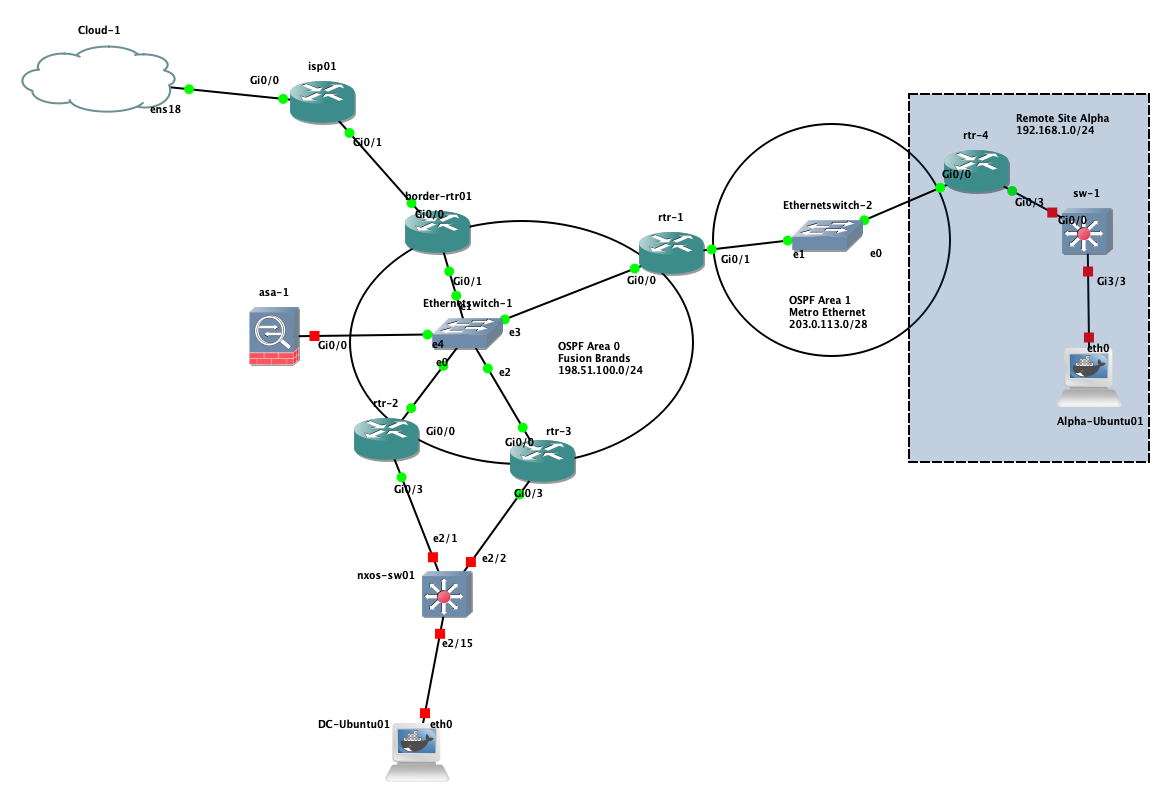
\includegraphics[width=\textwidth]{assets/base_setup.png}
    
\end{frame}

\begin{frame}[fragile]
    \frametitle{Playbook Management Key Values}
    All Ansible playbooks are defined within YAML format. Leveraging key/value
    pair assignments. We will take a look at some common keys used, and what their
    corresponding value looks like.
\begin{verbatim}
- name: "PLAY 1: Gather data from router"
  connection: network_cli
  hosts: r1
  become: true
  become_method: enable
\end{verbatim}
\end{frame}

\begin{frame}
    \frametitle{Gathering Data from Cisco IOS Devices}
    There are two methods to gather data from IOS devices, using:
    \begin{itemize}
        \item<2-> \textbf{ios\_command}
        \item<3-> \textbf{cli\_command}
    \end{itemize}
\end{frame}

\begin{frame}
    \frametitle{ios\_command}
    This is used when working with Cisco IOS devices connecting with SSH.
    
\end{frame}


\end{document}